\begin{figure}
    \centering
    \begin{subfigure}{.7\textwidth}
        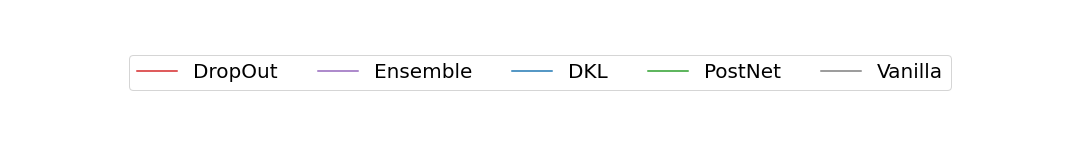
\includegraphics[width=\textwidth]{sections/011_icml2022/resources/legend-standard.png}
    \end{subfigure}
    \vspace{-3mm}
    
    \begin{subfigure}{.3\textwidth}
        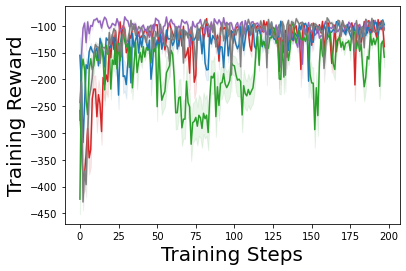
\includegraphics[width=\textwidth]{sections/011_icml2022/resources/acrobot-training_total_reward-training-model+.png}
    \end{subfigure}
    \begin{subfigure}{.3\textwidth}
        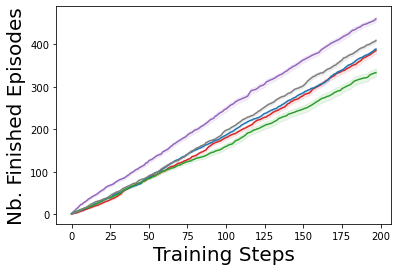
\includegraphics[width=\textwidth]{sections/011_icml2022/resources/acrobot-n_finished_training_episodes-training-model+.png}
    \end{subfigure}
    \begin{subfigure}{.3\textwidth}
        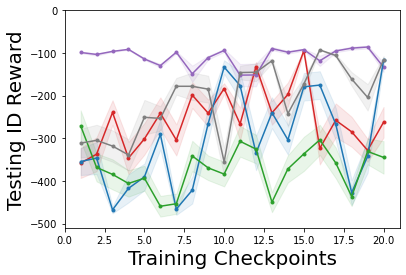
\includegraphics[width=\textwidth]{sections/011_icml2022/resources/Acrobot-v1-mean_reward_-testing-model+.png}
    \end{subfigure}

        \caption{Comparison of the vanilla DQN with the four uncertainty methods performance on Acrobot. All methods use the epsilon-greedy strategy. The vanilla DQN cannot be evaluated on uncertainty tasks.}
    \label{fig:camprison-vanilla-acrobot}
\end{figure}